%!TEX root = ./main.tex
\section{Derivation of Evaluation Rules}
\label{sec:ruleDerivation}

As discussed in the overview, frequent attempts on reverse desugaring during traditional resugaring processes is costive, so that making it inefficient. If we can statically derivate syntactic sugar's evaluation rules through its structure, it will greatly improve the efficiency of resugaring. In this section, we purpose such a method to make the resugaring of syntactic sugar more efficient.

Considering a simple syntactic sugar $\drule{(\m{not}~e_1)}{(\m{if}~e_1~\m{\#f}~\m{\#t})}$, obviously, we need to \textit{embed} the evaluation rules of \m{if} to get those of \m{not}. So we need a method that can express evaluation rules and is easy to transform. To accomplish these goals, we designed \textit{inference automaton} (IFA), which can be visually described by graphs.

Assuming that we already know the IFAs of all syntactic structures in CoreLang, the method of using IFA to construct the evaluation rules of syntactic sugar is as follows: First, construct the IFA of syntactic sugar according to the desugar rules. Then, transform and simplify IFA. Finally, generate evaluation rules for syntactic sugar.

In this section, we first give some examples of IFA and its formal definition. Then we introduce a more strict IFA called normal IFA. Next, we support an algorithm of conversion between evaluation rules and IFA. Finally, we discuss the role of IFA in dealing with syntactic sugar.

\subsection{Inference Automaton}

As mentioned above, IFA intuitively describes the evaluation rules of a certain syntactic structure. To help readers better understand it, we start with some examples, then we give the formal definition of IFA.

\subsubsection{IFA of \m{if}}

Considering evaluation rules of \m{if} in overview, we can observe that a term headed with \m{if} is first evaluated for $e_1$. Then it is chosen to evaluate $e_2$ or $e_3$ depending on the value of $e_1$. The evaluation result of $e_2$ or $e_3$ is the value of the term. Thus, we use Figure \ref{fig:ifa-if} to represent the evaluation rules of \m{if}.

\begin{figure}[t]
	\centering
	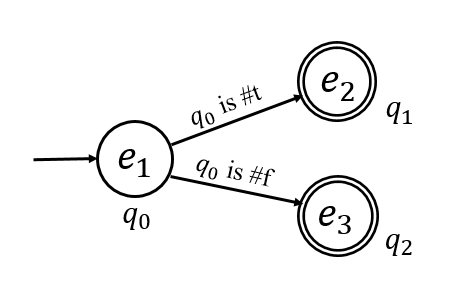
\includegraphics[scale=0.25]{images/ifa/ifa-if.png}
	\caption{IFA of \m{if}}
	\label{fig:ifa-if}
\end{figure}

A node of IFA indicates that the term needs to be evaluated, and the nodes before this have been evaluated. The arrow from $q_0$ to $q_1$ indicates that this branch is selected when the evaluation result of $e_1$ is \m{\#t}. The arrow between $e_1$ and $e_3$ is similar. The double circles of $e_2$ and $e_3$ denote that their evaluation result is the result of the term with this syntactic structure. In most cases, the transition condition is the evaluation result (an abstract value) of the previous node or a specific value. To simplify the representation of IFA in the figures of this paper, in the former case, we omit the condition on the transition edge; and in the latter case, we only mark the value on the transition edge.

When a term headed with \m{if} needs to be evaluated (for example \m{(if (if \#t \#t \#f) \#f \#t)}), first evaluating the $e_1$ (\m{(if \#t \#t \#f)}). Note that in this process, evaluating a subexpression requires running another automaton based on its syntax, while the outer automaton hold the state at $q_0$. According to the result of $e_1$ (\m{\#f}), the IFA selects the branch ($e_3$). Then the result of $e_3$ (\m{\#t}) is the evaluation result of the term.

\subsubsection{IFA of \m{nand}}

Sometimes the rules may be more complex, such as being reduced into another syntactic structure, or a term containing other syntactic structures. For example, we can express \m{nand}'s evaluation rules as follows. Based on the method discussed above, we can draw \m{nand}'s IFA as Figure \ref{fig:ifa-nand-a}.
\[
\infer{(\m{nand}~e_1~e_2) \to (\m{nand}~e_1'~e_2)}{e_1 \to e_1'}
\]\[
(\m{nand}~v_1~e_2) \to (\m{if}~(\m{if}~v_1~e_2~\m{\#f})~\m{\#f}~\m{\#t})
\]

% \infrule[E-Nand]{e_1 \to e_1'}{(\m{nand}~e_1~e_2) \to (\m{nand}~e_1'~e_2)}
% \infax[E-NandV]{(\m{nand}~v_1~e_2) \to (\m{if}~(\m{if}~v_1~e_2~\m{\#f})~\m{\#f}~\m{\#t})}

\begin{figure}[t]
\centering
\subcaptionbox{IFA according to the rules \label{fig:ifa-nand-a}}[.31\linewidth]{
    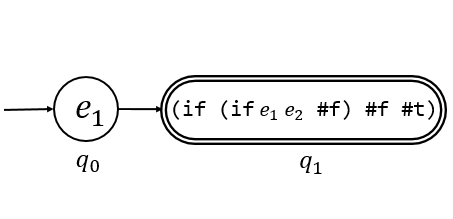
\includegraphics[scale=0.25]{images/ifa/ifa-nand-1-small.png}
}
\subcaptionbox{After expanding the outer \m{if} \label{fig:ifa-nand-b}}[.31\linewidth]{
    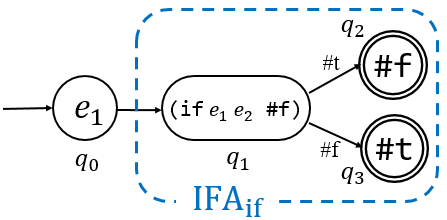
\includegraphics[scale=0.25]{images/ifa/ifa-nand-2-small.png}
}
\subcaptionbox{After expanding the inner \m{if} \label{fig:ifa-nand-c}}[.33\linewidth]{
    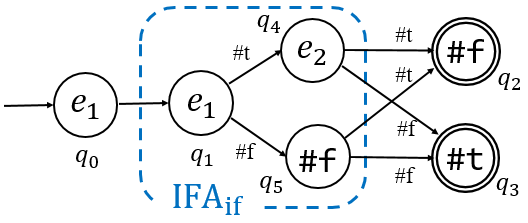
\includegraphics[scale=0.25]{images/ifa/ifa-nand-3-small.png}
}
\caption{IFA of \m{nand}}
\label{fig:ifa-nand}
\end{figure}

When the automaton runs into the terminal node of Figure \ref{fig:ifa-nand-a}, it derives the \m{if} term. In fact, we have known how \m{if} works through the IFA of \m{if}. Thus we can replace the last node with an $\text{IFA}_{\m{if}}$ and substitute $e_1$ to $e_3$ of $\text{IFA}_{\m{if}}$ with the parameters of the node. Use the termination nodes of $\text{IFA}_{\m{if}}$ as the termination nodes of new $\text{IFA}_{\m{nand}}$. The results are shown in Figure \ref{fig:ifa-nand-b}. Further decomposing the inner \m{if} node, connecting the terminating nodes of $\text{IFA}_{\m{nand}}$ to the nodes pointed to by the original output edge, we get Figure \ref{fig:ifa-nand-c}. 

As can be seen, the nodes of IFA in Figure \ref{fig:ifa-nand-c} have no other composite syntactic structures. Such an IFA completely expresses the semantics of a syntactic structure, and no longer cares about the evaluation rules of other syntactic structures. We do similar steps for syntactic sugar, which will be discussed later.

\subsubsection{IFA of \m{and}}

We represent the evaluation rule of \m{and} in a more complex way, as follows. 
\[
(\m{and}~e_1~e_2) \to (\m{let}~x~e_1~(\m{if}~x~e_2~x))
\]
In this case, we use the let binding. So we need to record the term represented by each variable at each node called symbol table. The representation of $\text{IFA}_{\m{and}}$ is shown in Figure \ref{fig:ifa-and-a}. 

Further discuss the syntactic structure. We first evaluate $e_1$ and save the result in $x$. When evaluating the term of \m{if}, what is actually evaluated is $(\m{if}~x~e_2~x)[e_1/x]$. We represent it in the form of Figure \ref{fig:ifa-and-b}, where node $q_1$ contains a symbol table for recording variables and the nodes referred to. It is similar to context, but since we mapped the variable to the node, we distinguished it. Mapping to nodes is to ensure that the variable data will not be lost when the IFA is transformed.

\begin{figure}[t]
\centering
\subcaptionbox{IFA according to the rules \label{fig:ifa-and-a}}[.4\linewidth]{
    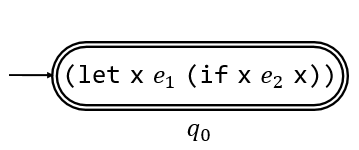
\includegraphics[scale=0.25]{images/ifa/ifa-and-1.png}
}
\subcaptionbox{After expanding \m{let} \label{fig:ifa-and-b}}[.4\linewidth]{
    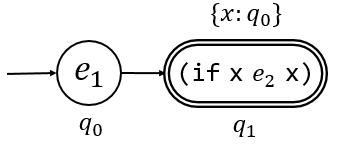
\includegraphics[scale=0.25]{images/ifa/ifa-and-2.png}
}
\caption{IFA of \m{and}}
\label{fig:ifa-and}
\end{figure}

%--------------------------------
\subsubsection{Definition of IFA}

\begin{Def}[Inference Automaton]

An inference automaton (IFA) of syntactic structure \m{CoreHead} is a 5-tuple, $(Q, \Sigma, q_0, F, \delta)$, consisting of

\begin{itemize}
    \item A finite set of nodes $Q$, each node contains a expression and a symbol table. The symbol table maps a variable to a node.
    \item A finite set of conditions $\Sigma$
    \item A start node $q_0 \in Q$
    \item A set of terminal nodes $F \subseteq Q$ 
    \item A transition function $\delta: (Q-F) \times \Sigma' \to Q$ where $\Sigma' \subseteq \Sigma$
\end{itemize}

and for each node $q$, there is no sequence of conditions $C = (c_1,c_2,\ldots,c_n)\subseteq \Sigma^*$, which makes that after $q$ transfers sequentially according to $P$, it returns $q$.

\end{Def}

The last constraint requires that there be no circles in our IFA.

In IFA, state transition does not depend on input. The only input of IFA is the term to be evaluated with this syntactic structure. The state transition is through whether the term meets the condition. Note that IFA is associated with syntactic structure. At Each IFA only represents the current evaluation of a syntactic structure. The state indicates that some sub-expressions of the syntactic structure have been evaluated, and the rest have not.

%======================
\subsection{Normal IFA}

Although IFA can intuitively show the behavior of a syntactic structure for evaluation, IFA itself has a complicated form. For example, the IFA of a syntactic structure may contain other syntactic structures as shown in Figure \ref{fig:ifa-nand-a}. We try to deform and simplify IFA to make it easier to analyze.

\begin{Def}[Normal IFA]
\label{def:nmlifa}
If an IFA meets following constraints, we call it a normal IFA.
\begin{itemize}
    \item The expression of node $q \in Q$ can only be $e_i$ or a pattern variable. If it is a pattern variable, it cannot be in the symbol table of $q$.
    \item For any $q_1,q_2 \in Q$ and $c_1, c_2 \in \Sigma$, $\delta(q_1, c_1) \neq \delta(q_2, c_2)$.
    \item On each branch, each $e_i$ can only be evaluated once.
\end{itemize}
\end{Def}

If an IFA is normal, it means there are no more composite syntactic structures in it. And it is a tree structure. We  prove that it is always feasible to convert IFA to normal IFA.

\begin{mythm}[Normalizability of IFA]
\label{mythm:nmlifa}
An IFA can be transformed into a normal IFA, if the normal IFAs of all sub-syntactic structures in the IFA are known.
\end{mythm}

In order to prove this theorem, we give the following steps and prove their correctness.

%------------------------------------
\subsubsection{Transform into a Tree}

When evaluating a term, different branches do not influence each other. Therefore, a node with at least two sources can be cloned and applied to different branches as shown in Figure \ref{fig:nmlifa-tree}. Replace the node referenced by the branch with the cloned node in conditions and symbol tables. The correctness is obvious. In this way, we can transform an IFA into a tree so that it satisfies the second constraint of normal IFA.

\begin{figure}[t]
\centering
\subcaptionbox{Before\label{fig:nmlifa-tree-1}}[.45\linewidth]{
    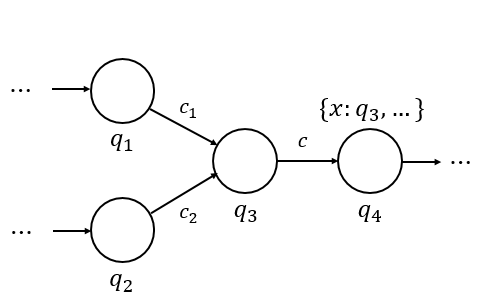
\includegraphics[scale=0.25]{images/nmlifa/nmlifa-tree-1.png}
}
\subcaptionbox{After\label{fig:nmlifa-tree-2}}[.45\linewidth]{
    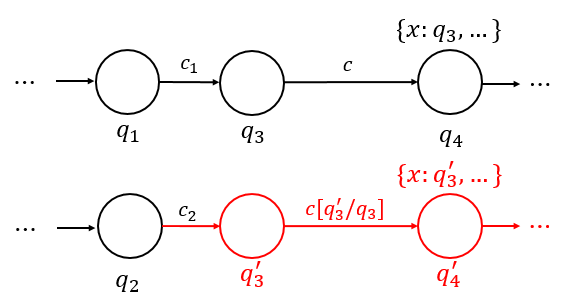
\includegraphics[scale=0.25]{images/nmlifa/nmlifa-tree-2.png}
}
\caption{Transform into a Tree}
\label{fig:nmlifa-tree}
\end{figure}

%-------------------------------------------------
\subsubsection{Substitute Sub-Syntactic Structure}

If the node $q$ in the tree IFA contains a term of a syntactic structure \m{H}, we replace this node with the IFA of \m{H}, replace the parameters and pass the symbol table of $q$ into the sub-IFA. Connect all the termination nodes of \m{H} to the original output node $q'$, and then convert it into a tree IFA according to the method described in the previous step as shown in Figure \ref{fig:nmlifa-subst}. Replace the node referenced by the branch with the \textit{new} one in conditions and symbol tables. This step can guarantee correctness, for $(\m{H}~e_1~\ldots~e_n)[e/x] = (\m{H}~e_1[e/x]~\ldots~e_n[e/x])$.

In particular, if we guarantee that a term $e$ does not contain a certain variable $x$, we can remove it from the symbol table. For example, in our problem, each $e_i$ of syntactic sugar cannot contain unbound variables. So we can remove all symbol tables of nodes with $e_i$.
\todo{@ziyi: declare handling on hygiene?}

\begin{figure}[t]
    \centering
    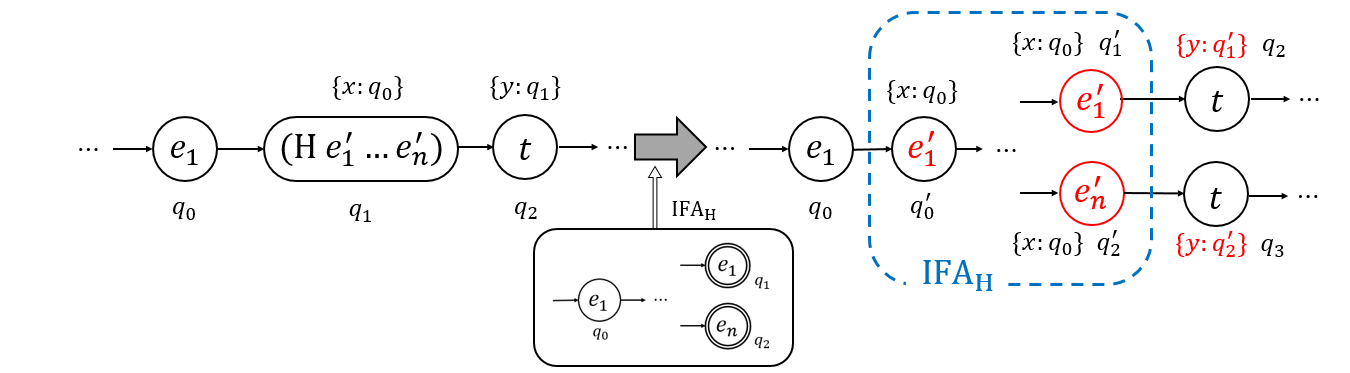
\includegraphics[scale=0.25]{images/nmlifa/nmlifa-subst.png}
    \caption{Substitute Sub-Syntactic Structure}
    \label{fig:nmlifa-subst}
\end{figure}

%----------------------------------------------------
\subsubsection{Replace Variables in the Symbol Table}

If the expression of a node $q$ is a pattern variable $x$ and $x$ is in the symbol table of $q$, we can replace $x$ with the expression of the node it points to, then remove $x$ from the symbol table as Figure \ref{fig:nmlifa-replace}. Because $x[e_1/x, e_2/y]=e_1[e_2/y]$, it is correct.

\begin{figure}[t]
\centering
\subcaptionbox{Before\label{fig:nmlifa-replace-1}}[.45\linewidth]{
    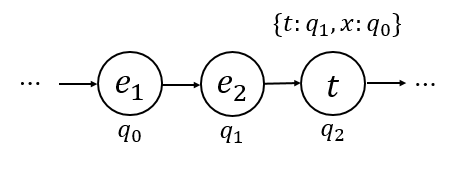
\includegraphics[scale=0.25]{images/nmlifa/nmlifa-replace-1.png}
}
\subcaptionbox{After\label{fig:nmlifa-replace-2}}[.45\linewidth]{
    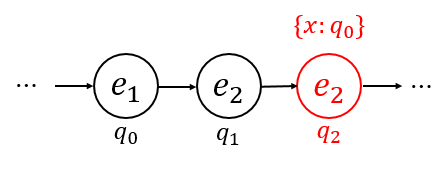
\includegraphics[scale=0.25]{images/nmlifa/nmlifa-replace-2.png}
}
\caption{Replace Variables in the Symbol Table}
\label{fig:nmlifa-replace}
\end{figure}

%---------------------------------------------------------------------
\subsubsection{Remove Evaluated Nodes and Merge Transition Conditions}

If an IFA is a tree, for each branch, remove the non-terminal nodes that have been evaluated with the same symbol table, and merge the conditions on the transition edge as Figure \ref{fig:nmlifa-merge}. Replace the node referenced by the branch with the first-evaluated node in conditions and symbol tables. This step can make an IFA satisfy the third constraint of normal IFA.
\todo{@ziyi: Remember ... is to verbally}

Since on any branch, if $e_i$ is removed, it must have been evaluated. Therefore, when IFA runs to this node, there is no need to do any evaluation on $e_i$. At the same time, the transfer edge ensures that the conditions are not lacking. Correctness is guaranteed.

\begin{figure}[t]
\centering
\subcaptionbox{Before\label{fig:nmlifa-merge-1}}[.45\linewidth]{
    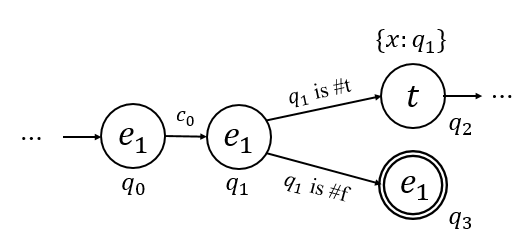
\includegraphics[scale=0.25]{images/nmlifa/nmlifa-merge-1.png}
}
\subcaptionbox{After\label{fig:nmlifa-merge-2}}[.45\linewidth]{
    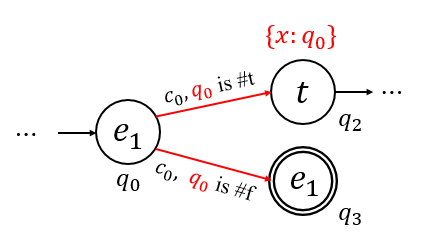
\includegraphics[scale=0.25]{images/nmlifa/nmlifa-merge-2.png}
}
\caption{Remove Evaluated Nodes and Merge Transition Conditions}
\label{fig:nmlifa-merge}
\end{figure}

%------------------------------------
\subsubsection{Remove Constant Value}

If the expression of a node is a constant value, remove the node and merge the conditions on the transition edge just like evaluated value. Because IFA does not do anything in this node, this does not affect the correctness of IFA.

%-------------------------------------
\subsubsection{Normalizability of IFA}

\begin{proof}[Proof of Theorem \ref{mythm:nmlifa}]
By repeating the above steps continuously, we can always get normal IFA. And it is equivalent to the original IFA for the correctness of each step.
\end{proof}

%===========================================
\subsection{Convert evaluation rules to IFA}

In the examples at the beginning of this section, we construct IFAs based on their semantics. Now, we give an algorithm that can automatically convert the evaluation rules to IFA and ensure its correctness. But at the same time, it has stricter requirements on the evaluation rules.

%--------------------------
\subsubsection{Assumptions}

\begin{Asm}
\label{Asm:rules}
A syntactic structure $CoreHead$ only contains the following evaluation rules.

\[
\infer
{(\m{CoreHead}~v_1\ldots v_p~e_1 \ldots e_i \ldots e_q) \to   (\m{CoreHead}~v_1\ldots v_p~e_1 \ldots e_i' \ldots e_q)}{e_i \to e_i'}
\]
\[
(\m{CoreHead}~v_1 \ldots v_p~e_1 \ldots e_q) \to e
\]

% \infrule[E-Head]
% {e_i \to e_i'}
% {(\m{CoreHead}~v_1\ldots v_p~e_1 \ldots e_i \ldots e_q) \to   (\m{CoreHead}~v_1\ldots v_p~e_1 \ldots e_i' \ldots e_q)}
% \infax[E-HeadR] {(\m{CoreHead}~v_1 \ldots v_p~e_1 \ldots e_q) \to e}

\end{Asm}

This assumption specifies the form of the evaluation rules to ensure that IFAs can be generated. The first one is a context rule, and the other one is a reduction rule. $e$ can be any value, one of the parameters or a term of another syntactic structure.

\begin{Asm}[Orderliness of Syntactic Structure]
\label{Asm:orderliness}
The syntactic structure in CoreLang is finite. Think of all syntactic structures as points in a directed graph. If one of $CoreHead$'s evaluation rules can generate a term containing $CoreHead'$, then construct an edge that points from $CoreHead$ to $CoreHead'$. The directed graph generated in this method has no circles.
\end{Asm}

IFAs are not able to construct syntactic structures that contain recursive rules. This assumption qualifies that we can find an order for all syntactic structures, and when we try to construct IFA for $CoreHead$, IFA of $CoreHead'$ is known.

\begin{Asm}[Determinacy of One-Step Evaluation]
\label{Asm:determinacy}
The rules satisfy the determinacy of one-step evaluation.
\end{Asm}

By assumption \ref{Asm:determinacy}, we can get the following lemma, which points out the feasibility of using a node in IFA to represent the evaluation of subexpressions.

\begin{lemma}
\label{lemma:one-step}
If a term $(\m{CoreHead}~e_1~\ldots~e_n)$ does a one-step evaluation by rule (E-Head) of $\m{CoreHead}$, which is a one-step evaluation of $e_i$, then it continues to use this rule until $e_i$ becomes a value.
\end{lemma}

\begin{proof}[Proof of Lemma \ref{lemma:one-step}]
According to Assumption \ref{Asm:determinacy}, this lemma is trivial.
\end{proof}

%------------------------
\subsubsection{Algorithm}

\begin{mythm}[IFA Can Be Constructed by Evaluation Rules]
\label{mythm:Rule2IFA}
If all the syntactic structures in CoreLang satisfy these assumptions, we can construct IFAs for all syntactic structures in CoreLang.
\end{mythm}

\begin{proof}[Proof of Theorem \ref{mythm:Rule2IFA}]

We prove this theorem by giving an algorithm that converts evaluation rules to IFA. By Assumption \ref{Asm:orderliness}, we get an order of syntactic structures. We construct the IFA for each structure in turn.

We generate a node for each rule of the syntactic structure \m{CoreHead} and insert them into $Q$. If the rule is a context rule for $e_i$, set $e_i$ as the expression of the node. If the rule is a reduction rule, add them into $F$ as terminal nodes and set the reduced term $e$ as the expression of the node. Symbol tables of these nodes are set to be empty. Next we connect these nodes.

For a term like $(\m{CoreHead}~e_1~\ldots~e_n)$, considering that $e_1\cdots e_n$ are not value, According to Lemma \ref{lemma:one-step}, we have the unique rule $r$ of \m{CoreHead} for one-step evaluation. Let node $q$ corresponding to $r$ be $q_0$.

If $r$ is a context rule for $e_i$, let the term of $q$ be $e_i$. Assume that the evaluation of $e_i$ results in $v_i$, we get term $(\m{CoreHead}~e_1 \ldots e_{i-1}~v_i~e_{i+1} \ldots e_n)$. For each possible value of $v_i$, choose the rules $r'$ that should be used. The node is $q'$. Set a condition as $c=q~\key{is}~v_i$ Let $\delta(q, c)$ be $q'$. For each branch, seem $r'$ as $r$ and keep doing this until $r$ is a reduction rule.

\end{proof}

In this way, we got an IFA of \m{CoreHead}. According to the lemma \ref{mythm:nmlifa}, we can also get a normal IFA of \m{CoreHead}. 

%---------------------------------------------------------
\subsubsection{Example: Construct IFA of \m{xor} by Rules}

We give an example to show how to convert evaluation rules to IFA using the algorithm mentioned above. Since the symbol tables of all nodes are empty, we omit not to write.

\infrule[E-Xor]{e_1 \to e_1'}{(\m{xor}~e_1~e_2) \to (\m{xor}~e_1'~e_2)}
\infax[E-XorTrue]{(\m{xor}~\m{\#t}~e_2) \to (\m{if}~e_2~\m{\#f}~\m{\#t})}
\infrule[E-XorFalse]{e_2 \to e_2'}{(\m{xor}~\m{\#f}~e_2) \to (\m{xor}~\m{\#f}~e_2')}
\infax[E-XorFalseTrue]{(\m{xor}~\m{\#f}~\m{\#t}) \to \m{\#t}}
\infax[E-XorFalseFalse]{(\m{xor}~\m{\#f}~\m{\#f}) \to \m{\#f}}

Suppose that \m{xor} is a syntactic structure in CoreLang. There are five rules for it. Therefore, we construct five nodes for the rules and set the expression as Figure \ref{fig:ifa-xor-a}.

Considering a term $(\m{xor}~e_1~e_2)$, where $e_1$ and $e_2$ are not values. It will be derived by rule (E-Xor). Therefore, set the node of the rule as the start node $q_0$. According to the rules of \m{xor}, the evaluation result of $e_1$ can be \m{\#t} or \m{\#f}. If the value is \m{\#t}, the term will be $(\m{xor}~\m{\#t}~e_2)$ and use rule (E-XorTrue) to derive. Then connect $q_0$ and $q_1$ with condition $q_0~\key{is}~\m{\#t}$. Connect $q_0$ and $q_2$ with condition $q_0~\key{is}~\m{\#f}$ similarly as Figure \ref{fig:ifa-xor-b}. Then connect $q_2$ to the last two nodes with conditions according to the value of $e_2$. The IFA of \m{xor} can be expressed as Figure \ref{fig:ifa-xor-c}.

\begin{figure}[t]
\centering
\subcaptionbox{\label{fig:ifa-xor-a}}[.3\linewidth]{
    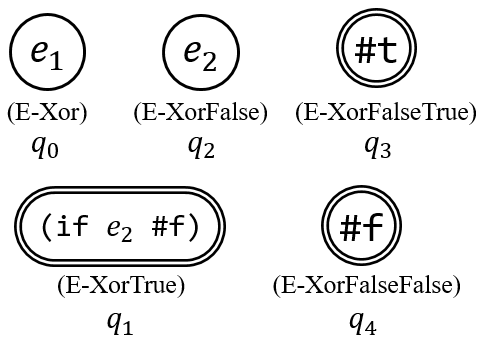
\includegraphics[scale=0.22]{images/ifa/ifa-xor-1.png}
}
\subcaptionbox{\label{fig:ifa-xor-b}}[.33\linewidth]{
    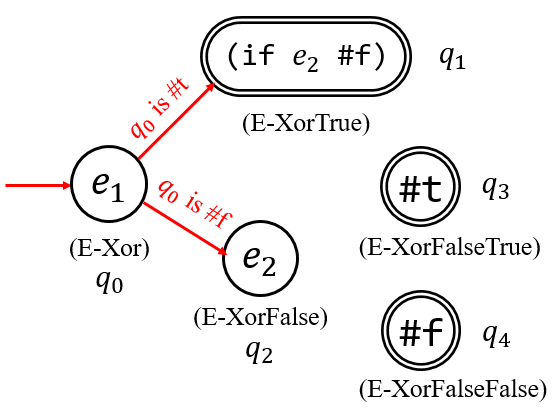
\includegraphics[scale=0.22]{images/ifa/ifa-xor-2.png}
}
\subcaptionbox{\label{fig:ifa-xor-c}}[.33\linewidth]{
    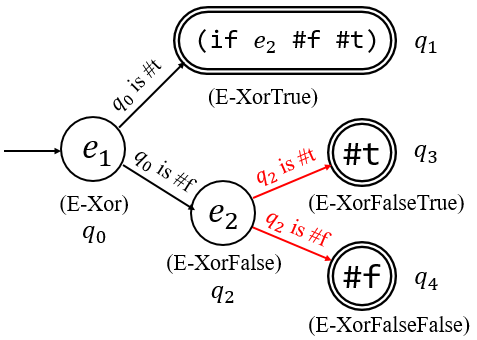
\includegraphics[scale=0.22]{images/ifa/ifa-xor-3.png}
}
\caption{IFA of \m{xor}: Constructed by evaluation rules}
\label{fig:ifa-xor}
\end{figure}

%--------------------------
\subsubsection{Correctness}

Before proving the correctness of the algorithm, we first prove the following lemma.

\begin{lemma}
\label{lemma:accessibility}
If a term $e$ of syntactic structure \m{CoreHead} uses rule $r$ to derive, we can find a path from $q_0$ to $q$ generated by $r$.
\end{lemma}

\begin{proof}[Proof of Lemma \ref{lemma:accessibility}]
Suppose $e=(\m{CoreHead}~v_1~\ldots~v_p~e_1~\ldots~e_q)$. We build a term $e_0'=(\m{CoreHead}~\m{id}(v_1)~\ldots~\m{id}(v_p)~e_1~\ldots~e_q)$, where $\m{id}(x)=x$. $e_0'$ should have the same value as $e$. If $e_0'$ is derived by rule $r_1$, $r_1$ must be a context rule, or $e$ can also be reduced by $r_1$. Also, the node $q_1$ generated by $r_1$ will be the start node. Without loss of generality, assume that $r_1$ is a context rule for $e_1$. We get $e_1'=(\m{CoreHead}~v_1~\m{id}(v_2)~\ldots~\m{id}(v_p)~e_1~\ldots~e_q)$ after derived by $r_1$. Similarly, we find a rule $r_2$ which is a context rule for $e_2$. The node $q_2$ generated by $r_2$ satisfies $\delta(q_1, (e_1~\key{is}~v_1))=q_2$. By analogy, we can get $e_p'=(\m{CoreHead}~v_1~\ldots~v_p~e_1~\ldots~e_q)=e$ and a path $q_1(=q_0), q_2, \ldots, q_p$. At last, we use rule $r$ to derive $e$ and add $q$ to the path.
\end{proof}

\begin{lemma}
\label{lemma:rule2ifa-correct}
For any syntactic structure \m{CoreHead}, if its evaluation rules meets the above assumptions, the normal IFA got by the algorithm in Theorem \ref{mythm:Rule2IFA} has the same semantics as the rules. 
\end{lemma}

In other words, for any term of syntactic structure \m{CoreHead}, evaluating the term by IFA and evaluating by rule get the same derivation sequence.

\begin{proof}[Proof of Lemma \ref{lemma:rule2ifa-correct}]
We only need to discuss that in a one-step derivation, both get the same result.

Considering a term $e=(\m{CoreHead}~e_1 \ldots e_n)$ use rule $r$ to derive. Suppose $r$ generate node $q$. By Lemma \ref{lemma:accessibility}, we find a path from $q_0$ to $q$. The term $e$ must meet the conditions from $q_0$ to $q$. Therefore, the one-step derivation of this term $e$ in IFA must be located at $q$. If $r$ is a context rule for $e_i$, the expression of $q$ is $e_i$ as well, and $e_i$ of $e$ is not a value. Thus both of the one-step derivation of $e$ are one-step derivation of $e_i$. If $r$ is a reduction rule to $e'$, both of them are $e'$.

Similarly, if an term can be derived in one step in IFA, then it must be able to use the corresponding rule for one-step derivation.
]
\end{proof}

%-----------------------------
\subsubsection{IFA of \m{let}}

If a certain syntactic structure does not meet the above assumptions, it does not mean that this syntactic structure does not have an IFA. We can define its IFA according to its semantics. However, this method cannot be automated and requires users to ensure its correctness. For example, given the evaluation rules of \m{let}, we can specify the IFA of \m{let} as Figure \ref{fig:ifa-let}.
\[
\infer{\m{let}~x~e_1~e_2 \to \m{let}~x~e_1'~e_2}{e_1 \to e_1'}
\]\[
(\m{let}~x~e_1~e_2) \to e_2[e_1/x]
\]

% \infrule[E-Let]{e_1 \to e_1'}{\m{let}~x~e_1~e_2 \to \m{let}~x~e_1'~e_2}
% \infax[E-LetSubst]{(\m{let}~x~e_1~e_2) \to e_2[e_1/x]}

\begin{figure}[t]
    \centering
    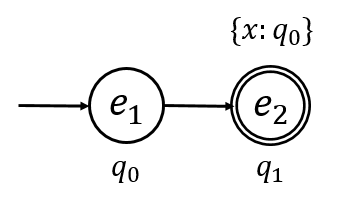
\includegraphics[scale=0.25]{images/ifa/ifa-let.png}
    \caption{IFA of \m{let}}
    \label{fig:ifa-let}
\end{figure}

In the evaluation rules of \m{let}, there is a substitution. Therefore, in IFA of \m{let}, we need symbol table to express this. When $e_2$ is evaluated or expanded, it is necessary to replace $x$ with the value of node $q_0$ in $e_2$.




%===========================================
\subsection{Convert IFA to Evaluation Rules}

Next we try to convert IFA to evaluation rules. Because IFA can be converted into normal IFA by Theorem \ref{mythm:nmlifa}, we only need to convert normal IFA into rules. Unfortunately, IFA can express some derivation methods whose evaluation rules are difficult to describe. Therefore, we also need to have stricter constraints on IFA to ensure that evaluation rules can be generated.

\begin{Asm}
\label{Asm:st} 
In a normal IFA, if $q \notin F$, then the symbol table of $q$ is empty, and the expression of $q$ cannot be pattern variable.
\end{Asm}

In fact, this is a very strong assumption, which requires that only termination nodes could have substitution. Because it is difficult for us to generate a context rule for the term after substitution.

%------------------------
\subsubsection{Algorithm}

Similarly, we first give its algorithm, and then prove its correctness.

\begin{mythm}[Rules Can Be Constructed by Normal IFA]
\label{mythm:ifa2rule}
For each normal IFA satisfy Assumption \ref{Asm:st}, it can be converted to evaluation rules.
\end{mythm}

\begin{proof}[Proof of Theorem \ref{mythm:ifa2rule}]

Suppose that the IFA stands for the syntactic structure $H$, then we build evaluation rules for $H$. First traverse all nodes to find the set of all terms in nodes, which is the parameters of the syntactic structure $H$ like $(\m{H}~e_1 \ldots e_n)$. Then generate evaluation rule for each node.

Begin with $q_0$, traverse the IFA. Let $q$ be $q_0$. Record the conditions by a set $T$.

Suppose that $q$ is a terminal node, the expression of $q$ is $e$ and the symbol table of $q$ is like $\{x:q_x; y:q_y; \ldots\}$. Let $e_x,e_y,\ldots$ be the expressions of $q_x, q_y, \ldots$. Add a reduction rule like
\[
\infer{(\m{H}~e_1 \ldots e_n) \to e[e_x/x][e_y/y]\ldots}{T}
\]
% \infrule[E-Hr]{T}{(\m{H}~e_1 \ldots e_n) \to e[e_x/x][e_y/y]\ldots}

If $q$ is not a termination node, and the expression of $q$ is $e_i$, add a context rule like
\[
\infer{(\m{H}~e_1~\ldots~e_i~\ldots~e_n) \to (\m{H}~e_1~\ldots~e_i'~\ldots~e_n)}{e_i \to e_i' \quad T}
\]

%\infrule[E-Hi]{e_i \to e_i' \quad T}{(\m{H}~e_1~\ldots~e_i~\ldots~e_n) \to (\m{H}~e_1~\ldots~e_i'~\ldots~e_n)}

For each condition $c$ and node $q'$ satisfying $\delta(q, c)=q'$, do the following steps separately. Replace the node in $c$ with its expression and add it to $T$. Let $q'$ be $q$. Keep doing this until $q$ is a terminal node.

\end{proof}

%----------------------------------------------------------
\subsubsection{Example: Construct Rules of \m{nand} by IFA}

Figure \ref{fig:ifa-nand-bs} is the IFA of \m{nand} which have been constructed. We can simplify it and get a normal IFA as Figure \ref{fig:ifa-nand-as}.

\begin{figure}[t]
\centering
\subcaptionbox{Before Simplification\label{fig:ifa-nand-bs}}[.45\linewidth]{
    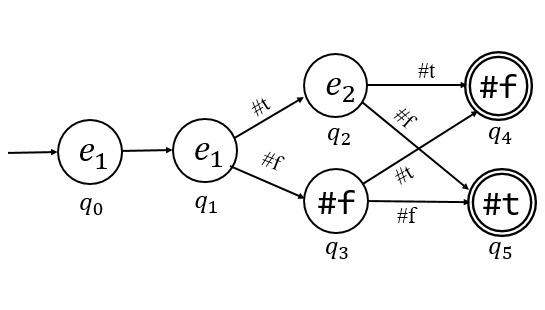
\includegraphics[scale=0.28]{images/ifa/ifa-nand-4.png}
}
\subcaptionbox{After Simplification\label{fig:ifa-nand-as}}[.45\linewidth]{
    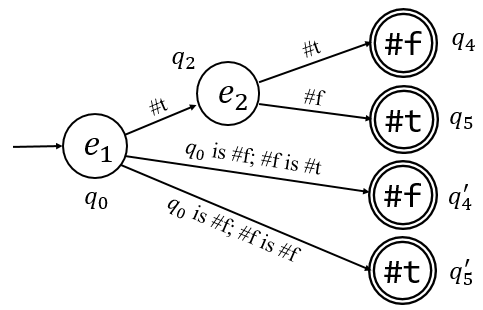
\includegraphics[scale=0.28]{images/ifa/ifa-nand.png}
}
\caption{IFA of \m{nand}}
\label{fig:ifa-nand-std}
\end{figure}

Start with $q_0$, we get a context rule as
\[
\infer{(\m{nand}~e_1~e_2) \to (\m{nand}~e_1'~e_2)}{e_1 \to e_1'}
\]
% \infrule[E-Nand]{e_1 \to e_1'}{(\m{nand}~e_1~e_2) \to (\m{nand}~e_1'~e_2)}

We first discuss the branch of $q_2$. Add $e_1 \key{is} \m{\#t}$ to $T$. Because $q_2$ is not a terminal node, add a new context rule for $q_2$.
\[
\infer{(\m{nand}~e_1~e_2) \to (\m{nand}~e_1~e_2')}{e_2 \to e_2'\quad e_1~\key{is}~\m{\#t}}
\]
% \infrule[E-NandTrue]{e_2 \to e_2'\quad e_1~\key{is}~\m{\#t}}{(\m{nand}~e_1~e_2) \to (\m{nand}~e_1~e_2')}

Since $q_4$ is a reduction rule, append $e_2 \key{is} \m{\#t}$ to $T$ and add a new reduction rule for $q_4$. Reduction rule for $q_5$ is similar.
\[
\begin{array}{c}
\infer{(\m{nand}~e_1~e_2) \to \m{\#f}}{e_1~\key{is}~\m{\#t}\quad e_2~\key{is}~\m{\#t}}
\quad
\infer{(\m{nand}~e_1~e_2) \to \m{\#t}}{e_1~\key{is}~\m{\#t}\quad e_2~\key{is}~\m{\#f}}
\end{array}
\]
% \infrule[E-NandTrueTrue]{e_1~\key{is}~\m{\#t}\quad e_2~\key{is}~\m{\#t}}{(\m{nand}~e_1~e_2) \to \m{\#f}}
% \infrule[E-NandTrueFalse]{e_1~\key{is}~\m{\#t}\quad e_2~\key{is}~\m{\#f}}{(\m{nand}~e_1~e_2) \to \m{\#t}}

Back to $q_0$, for $q_4'$ and $q_5'$ are also terminal nodes, we can build reduction rules for $q_4'$ and $q_5'$ in the same way.
\[
\begin{array}{c}
\infer{(\m{nand}~e_1~e_2) \to \m{\#f}}{e_1~\key{is}~\m{\#f}\quad \m{\#f}~\key{is}~\m{\#t}}
\quad
\infer{(\m{nand}~e_1~e_2) \to \m{\#t}}{e_1~\key{is}~\m{\#f}\quad \m{\#f}~\key{is}~\m{\#f}}
\end{array}
\]
% \infrule[E-NandFalse1]{e_1~\key{is}~\m{\#f}\quad \m{\#f}~\key{is}~\m{\#t}}{(\m{nand}~e_1~e_2) \to \m{\#f}}
% \infrule[E-NandFalse2]{e_1~\key{is}~\m{\#f}\quad \m{\#f}~\key{is}~\m{\#f}}{(\m{nand}~e_1~e_2) \to \m{\#t}}

We can judge that \m{\#f} is not \m{\#t}, so we can remove the rule (NandFalse1) from the rules, for it contains a condition that is never met. At the same time, we rewrite the remaining rules into a more customary form.
\[
\begin{array}{cc}
\infer{(\m{nand}~e_1~e_2) \to (\m{nand}~e_1'~e_2)}{e_1 \to e_1'}
&
\infer{(\m{nand}~\m{\#t}~e_2) \to (\m{nand}~\m{\#t}~e_2')}{e_2 \to e_2'}
\end{array}
\]\[
\begin{array}{ccc}
(\m{nand}~\m{\#t}~\m{\#t}) \to \m{\#f}
&
(\m{nand}~\m{\#t}~\m{\#f}) \to \m{\#t}
&
(\m{nand}~\m{\#f}~e_2) \to \m{\#t}
\end{array}
\]

% \infrule[E-Nand]{e_1 \to e_1'}{(\m{nand}~e_1~e_2) \to (\m{nand}~e_1'~e_2)}
% \infrule[E-NandTrue]{e_2 \to e_2'}{(\m{nand}~\m{\#t}~e_2) \to (\m{nand}~\m{\#t}~e_2')}
% \infax[E-NandTrueTrue]{(\m{nand}~\m{\#t}~\m{\#t}) \to \m{\#f}}
% \infax[E-NandTrueFalse]{(\m{nand}~\m{\#t}~\m{\#f}) \to \m{\#t}}
% \infax[E-NandFalse]{(\m{nand}~\m{\#f}~e_2) \to \m{\#t}}


%--------------------------
\subsubsection{Correctness}

\begin{lemma}
\label{lemma:ifa2rule-correct}
For any syntactic structure \m{H}, if its normal IFA meets the above assumptions, the evaluation rules obtained according to the algorithm in Theorem \ref{mythm:ifa2rule} have the same semantics as IFA. 
\end{lemma}

In other words, for any term of syntactic structure \m{H}, evaluating the term by IFA and evaluating by rule get the same derivation sequence.

\begin{proof}[Proof of Lemma \ref{lemma:ifa2rule-correct}]
We only need to discuss that in a one-step derivation, both get the same result.

Considering a term $e=(\m{H}~e_1 \ldots e_n)$ use rule $r$ to derive. The term $e$ must meet the condition $T$ of $r$ such as some parameters must be value or a specific value. Suppose $r$ is generated by node $q$. Then $T$ is the set of all transition conditions from $q_0$ to $q$. Therefore, the one-step derivation of this term $e$ in IFA must be located at $q$. If $r$ is a context rule for $e_i$, the expression of $q$ is $e_i$ as well, and $e_i$ of $e$ is not a value. Thus both of the one-step derivation of $e$ are one-step derivation of $e_i$.

Similarly, if an term can be derived in one step in IFA, then it must be able to use the corresponding rule for one-step derivation.

\end{proof}

%===========================
\subsection{Syntactic Sugar}

We can find that although rules of \m{nand} we used when constructing the IFA included the syntactic structure of \m{if}, the final result does not. For syntactic sugar, we also deal with it with a similar idea, that is, construct the IFA of syntactic sugar, simplify it and convert it into rules. With the IFA, we can easily get the evaluation rules for syntactic sugars.

Similarly, we also need to add some constraints on syntactic sugar.

\begin{Asm}[Orderliness of Syntactic Sugar]
\label{Asm:orderliness-sugar}
The definition of each syntactic sugar can only use the syntactic structure in coreLang and the syntactic sugar that has been defined.
\end{Asm}

\begin{Def}
\label{def:ifa-sugar}
Considering the following syntactic sugar 
\[
\drule{(\m{SurfHead}~x_1~\ldots~x_n)}{e},
\] 
the IFA of \m{SurfHead} is defined as the IFA of syntactic structure \m{SurfHead'} whose evaluation rule is
\[
(\m{SurfHead'}~x_1~\ldots~x_n) \to e
\]

\end{Def}

%--------------------------------------------
\subsubsection{An Example of Syntactic Sugar}

Suppose that there are only \m{if} and \m{let} in our CoreLang, whose IFAs are known. Now we build rules for syntactic sugar \m{or} and \m{sg}.
\[
\drule{(\m{or}~e_1~e_2)}{(\m{let}~x~e_1~(\m{if}~x~x~e_2))} 
\]

\m{or} syntactic sugar only uses the syntax structure of CoreLang, which meets Assumption \ref{Asm:orderliness-sugar}. Then we generate evaluation rules for \m{or}.

\begin{figure}[t]
    \centering
    \subcaptionbox{Rule of Definition \ref{def:ifa-sugar} \label{fig:ifa-ex-or-1}}[.31\linewidth]{
        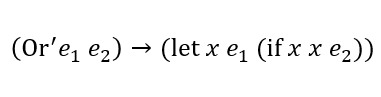
\includegraphics[scale=0.3]{images/ifa/ifa-ex-or-1.png}
    }
    \subcaptionbox{IFA generated with the algorithm of Theorem \ref{mythm:Rule2IFA} \label{fig:ifa-ex-or-2}}[.31\linewidth]{
        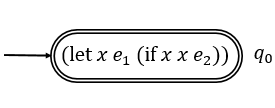
\includegraphics[scale=0.3]{images/ifa/ifa-ex-or-2.png}
    }
    \subcaptionbox{Expand syntactic structure of \m{let} \label{fig:ifa-ex-or-3}}[.31\linewidth]{
        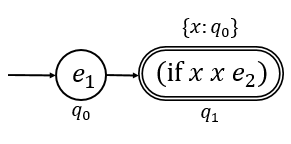
\includegraphics[scale=0.3]{images/ifa/ifa-ex-or-3.png}
    }
    \subcaptionbox{Expand syntactic structure of \m{if} \label{fig:ifa-ex-or-4}}[.31\linewidth]{
        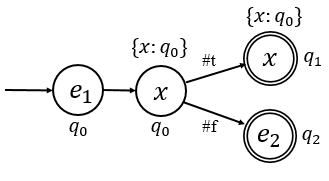
\includegraphics[scale=0.3]{images/ifa/ifa-ex-or-4.png}
    }
    \subcaptionbox{Replace $x$ with expression according to the symbol table \label{fig:ifa-ex-or-5}}[.31\linewidth]{
        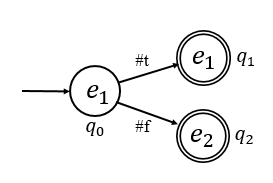
\includegraphics[scale=0.3]{images/ifa/ifa-ex-or-5.png}
    }
    \subcaptionbox{Rules generated with the algorithm of Theorem \ref{mythm:ifa2rule} \label{fig:ifa-ex-or-6}}[.31\linewidth]{
        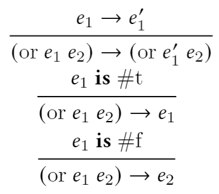
\includegraphics[scale=0.3]{images/ifa/ifa-ex-or-6.png}
    }
    \caption{Example: Syntactic Sugar of \m{or}}
    \label{fig:ifa-nand-std}
\end{figure}

The IFA of \m{or} is the same as the IFA of \m{or'} whose rule is shown in Figure \ref{fig:ifa-ex-or-1}. Therefore, we can generate an IFA according to the rule as shown in Figure \ref{fig:ifa-ex-or-2}. Next we transform IFA to make it a normal IFA, as shown in Figure \ref{fig:ifa-ex-or-3} to Figure \ref{fig:ifa-ex-or-5}. Finally, according to the structure of IFA, generate or evaluation rules, as shown in Figure \ref{fig:ifa-ex-or-6}.

% \infrule[E-Or]{e_1 \to e_1'}{(\m{or}~e_1~e_2) \to (\m{or}~e_1'~e_2)}
% \infrule[E-OrTrue]{e_1~\key{is}~\m{\#t}}{(\m{or}~e_1~e_2) \to e_1}
% \infrule[E-OrFalse]{e_1~\key{is}~\m{\#f}}{(\m{or}~e_1~e_2) \to e_2}

%--------------------------
\subsubsection{Correctness}

As discussed in Section \ref{sec3}, our approach should satisfy the three properties: emulation, abstraction and coverage. The property of abstraction is obvious, for the rules we generate only contain the syntactic structure itself, without any other structures in core language. However, our approach does not perfectly satisfy emulation and coverage. In the derivation, we lost the information that a syntactic structure is reduced to another syntactic structure. This makes the derivation sequence different. But through Theorem \ref{mythm:nmlifa}, Lemma \ref{lemma:rule2ifa-correct} and Lemma \ref{lemma:ifa2rule-correct}, we can guarantee the correctness of the evaluation results.








